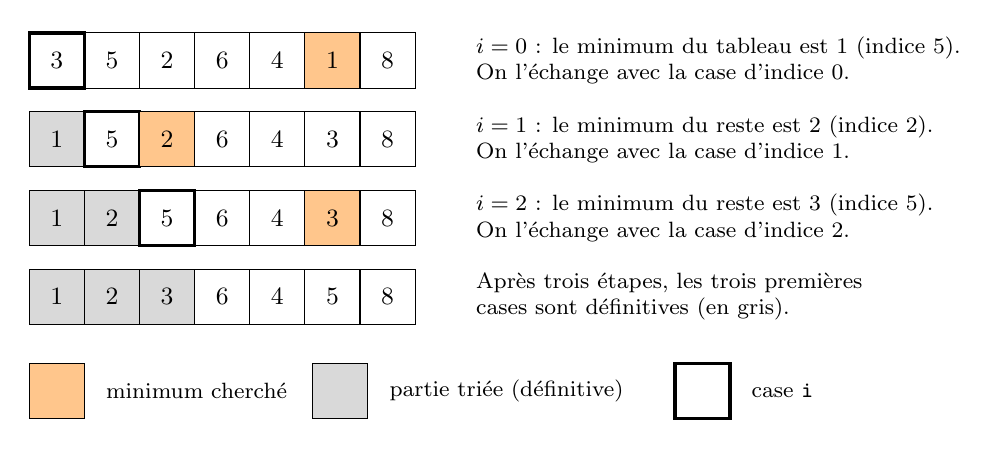
\begin{tikzpicture}[x=1cm,y=1cm,c/.style={draw,minimum size=0.7cm,inner sep=0pt,font=\small},
 mn/.style={fill=orange!45},ok/.style={fill=gray!30},cl/.style={fill=cyan!30},ix/.style={thick,draw=black,line width=1.2pt},hors/.style={text=gray,draw=gray!60},lab/.style={anchor=west,font=\footnotesize,align=left}]
\node[c,ix] at (0.00,0.00) {3};
\node[c,] at (0.70,0.00) {5};
\node[c,] at (1.40,0.00) {2};
\node[c,] at (2.10,0.00) {6};
\node[c,] at (2.80,0.00) {4};
\node[c,mn] at (3.50,0.00) {1};
\node[c,] at (4.20,0.00) {8};
\node[lab] at (5.2,0.00) {$i=0$ : le minimum du tableau est $1$ (indice 5).\\On l'échange avec la case d'indice 0.};
\node[c,ok] at (0.00,-1.00) {1};
\node[c,ix] at (0.70,-1.00) {5};
\node[c,mn] at (1.40,-1.00) {2};
\node[c,] at (2.10,-1.00) {6};
\node[c,] at (2.80,-1.00) {4};
\node[c,] at (3.50,-1.00) {3};
\node[c,] at (4.20,-1.00) {8};
\node[lab] at (5.2,-1.00) {$i=1$ : le minimum du reste est $2$ (indice 2).\\On l'échange avec la case d'indice 1.};
\node[c,ok] at (0.00,-2.00) {1};
\node[c,ok] at (0.70,-2.00) {2};
\node[c,ix] at (1.40,-2.00) {5};
\node[c,] at (2.10,-2.00) {6};
\node[c,] at (2.80,-2.00) {4};
\node[c,mn] at (3.50,-2.00) {3};
\node[c,] at (4.20,-2.00) {8};
\node[lab] at (5.2,-2.00) {$i=2$ : le minimum du reste est $3$ (indice 5).\\On l'échange avec la case d'indice 2.};
\node[c,ok] at (0.00,-3.00) {1};
\node[c,ok] at (0.70,-3.00) {2};
\node[c,ok] at (1.40,-3.00) {3};
\node[c,] at (2.10,-3.00) {6};
\node[c,] at (2.80,-3.00) {4};
\node[c,] at (3.50,-3.00) {5};
\node[c,] at (4.20,-3.00) {8};
\node[lab] at (5.2,-3.00) {Après trois étapes, les trois premières\\cases sont définitives (en gris).};
\node[c,mn] at (0,-4.2){};\node[lab] at (0.5,-4.2){minimum cherché};\node[c,ok] at (3.6,-4.2){};\node[lab] at (4.1,-4.2){partie triée (définitive)};\node[c,ix] at (8.2,-4.2){};\node[lab] at (8.7,-4.2){case \texttt{i}};
\end{tikzpicture}